\subsection{Frontend: Benutzerschnittstelle}
Das in React geschriebene Frontend besteht aus einer Hauptkomponente, welche aus mehreren Kindkomponenten besteht (siehe Abbildung \ref{fig:frontend}).
Ein \textit{Header}, welcher die Möglichkeit bietet die Seite neuzuladen, Informationen über die Internetseite einzuholen und den Darkmode zu aktivieren, befindet sich am oberen Bildschirmrand.
Über ein Benutzersymbol, werden nach einer Autorisierung weitere Funktionalitäten für Entwickler freigeschalten.
Eine weitere Komponente im oberen Bereich ermöglicht dem Benutzer den Upload eines eigenen oder eines Beispielbildes.
Zwei weitere Komponenten am linken Bildschirmrand, \textit{Selected Image} und \textit{Imagedetails}, sind dafür zuständig das hochgeladene Bild anzuzeigen, sowie die Bildinformationen in Form eines Histogrammes anzuzeigen.
Die Komponente \textit{Availible steps} am rechten Bildschirmrand stellt dem Benutzer alle möglichen Bildoperationen zur Verfügung.
Möchte dieser eine Bildoperation anwenden, muss eine Karte aus der Komponente per Drag and Drop in die dafür vorgesehene Komponente \textit{Pipeline} im Zentrum gezogen werden.
Möchte der Benutzer die Verarbeitung starten, kann dieser das durch das Klicken der Schaltfläche \textit{Start Pipeline} erreichen.
Das Frontend schickt daraufhin alle benötigten Informationen an das Backend.
Das Klicken des Symbols \textit{i} bei einem Verarbeitungsschritt liefert dem Benutzer Informationen zu der jeweiligen Bildoperation.
Hat der Benutzer einen Verarbeitungsschritt abgelegt, kann er über das Klicken des nach unten gerichteten Pfeils die Parameter der Bildoperation konfigurieren.
Klickt der Benutzer auf das Sichbarkeitssymbol eines Verarbeitungsschritts, wird das Zwischenergebnis angezeigt.
Dies ermöglicht es dem Benutzer, Schritt für Schritt Ergebnisse aus den einzelnen Verarbeitungsschritten nachzuvollziehen.
\begin{figure*}[ht]
    \centering
    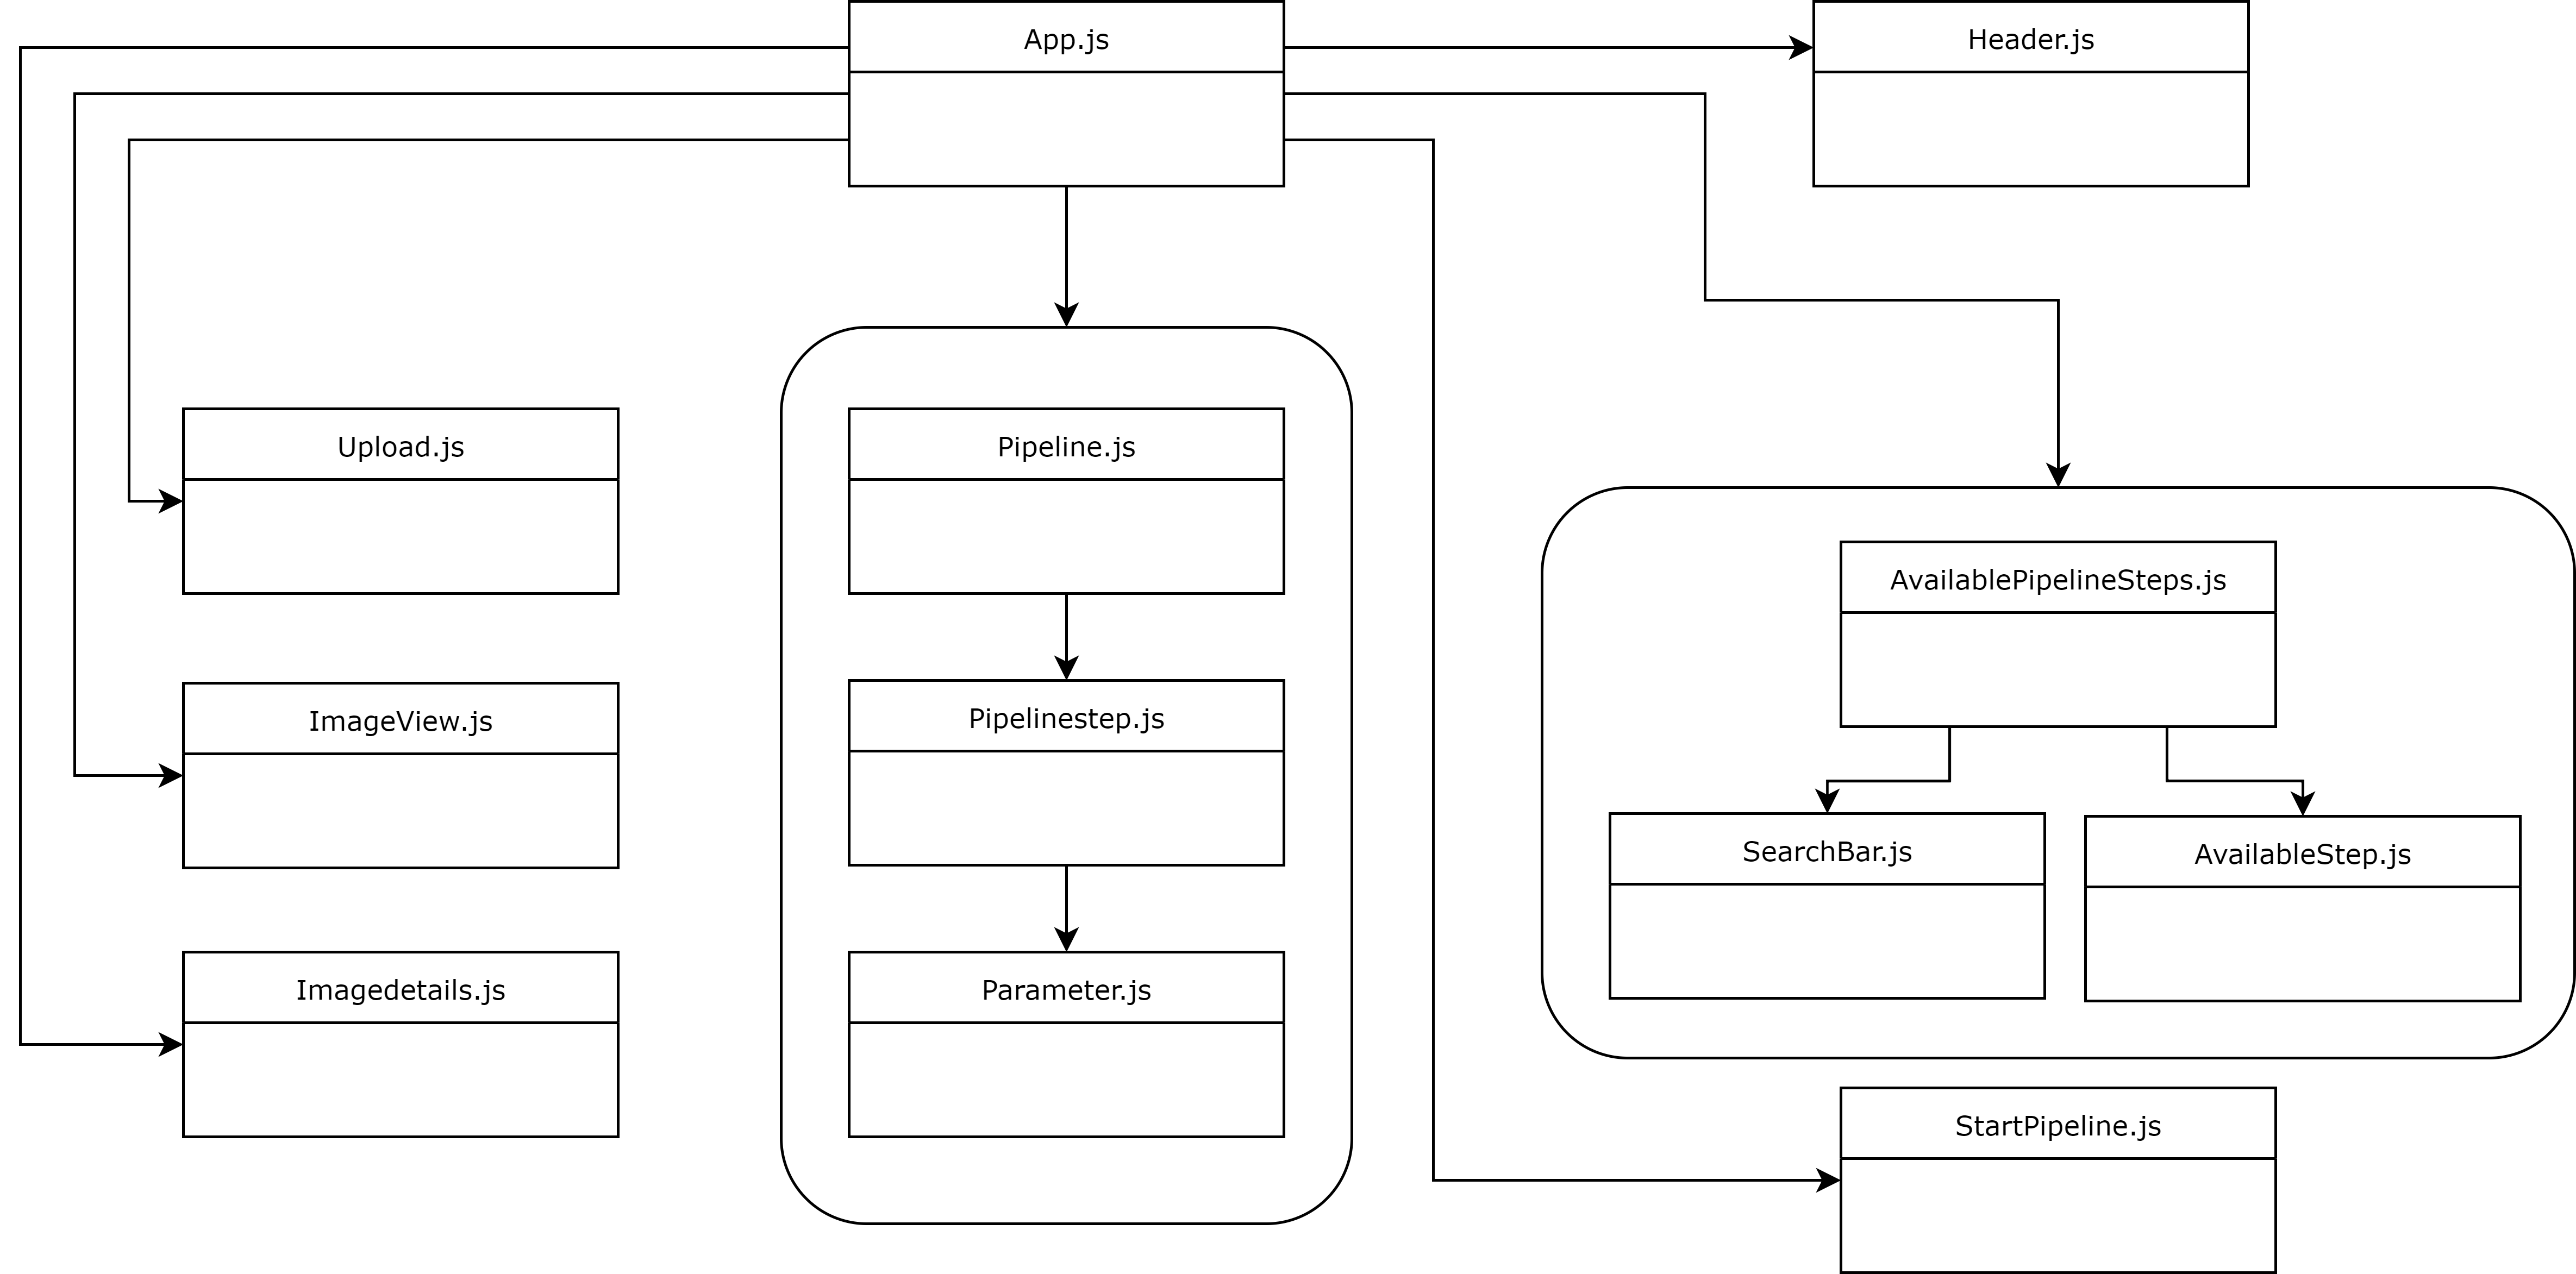
\includegraphics[width=\textwidth]{Bilder/FrontendBDCC.drawio.png}
    \caption{Übersicht der Komponenten im Frontend}
    \label{fig:frontend}
\end{figure*}